\section{*应用：透镜空间的同伦分类}
\sourcepage{489--490}
本节假定读者熟悉透镜空间（第 4.14 节）。上同调的杯积环结构通过 Poincaré 对偶同构，诱导同调上的环结构，称为\emph{同调交环}。在上同调被发现以前，这个环就已经为人所知。粗略地说，两个同调类的交积由代表它们的闭链的几何交定义。这样定义运算并推导性质，需要相当多工作。虽然运算是拓扑不变量，但一般连续映射即使在同维流形之间也不保持它。因此，把交积推广到任意多面体的努力未能成功，也并不令人意外。

今天我们把上同调环视为自然对象，把流形同调交环的存在看成由 Poincaré 对偶带来的有利现象。这里不详细研究交环，只证明一个把交积解释为闭链几何交的引理，以便计算透镜空间的上同调环。

\entry{记号}{8.9.1}本节 $X$ 始终为紧致连通、可三角剖分的 $n$ 维流形。若可定向，$\Gamma$ 为定向类，$R$ 为任意有单位元交换环；若不可定向，令 $\Gamma=\Gamma_{(2)}$，$R=\Z/2$。

\entry{定义}{8.9.2}对 $\alpha_p\in H_p(X;R)$、$\beta_q\in H_q(X;R)$，取唯一的类满足
\[\alpha^{n-p}\frown\Gamma=\alpha_p,\qquad\beta^{n-q}\frown\Gamma=\beta_q,\]
定义\emph{交积}
\[\alpha_p\cdot\beta_q=(\alpha^{n-p}\smile\beta^{n-q})\frown\Gamma.\]
可定向情形下结果的符号依赖于定向类。积的维数为 $p+q-n$，这与 $\R^n$ 中一般位置的 $p$ 维平面与 $q$ 维平面的交的维数相同，因而暗示它与几何交有关。

\entry{引理}{8.9.3}采用上述记号，设 $p+q=n$。类 $\alpha_p$ 由承载于对偶 $p$ 维骨架的重分后闭链 $c_p$ 代表，$\beta_q$ 由原复形的闭链 $d_q$ 代表。假设二者的承载集只交于一个 $q$ 维单形 $\sigma$ 的重心。若 $d_q$ 在 $\sigma$ 上的系数为 $\pm a$，$c_p$ 在对偶块 $D(\sigma)$ 上的系数为 $\pm b$，则其交积差一个符号由零维链 $ab\widehat\sigma$ 代表。

\sourcepage{491}
\textbf{证明：}取 $\alpha^q,\beta^p$ 为对应上同调类。由定义及帽积公式，
\[\alpha_p\cdot\beta_q=(\alpha^q\smile\beta^p)\frown\Gamma
=\alpha^q\frown\beta_q.\]
增广诱导 $H_0(X;R)\cong R$，故只需证明
\[\langle\alpha^q,\beta_q\rangle=\epsilon_*(\alpha_p\cdot\beta_q)=\pm ab.\]
取代表 $\Gamma$ 的顶维闭链 $\gamma$，并使用上一节构造的同构
\[\psi:C^q(X)\to\mathcal D_p(X),\qquad
j\psi(c^q)=g^\#c^q\frown\operatorname{sd}\gamma.\]
对有向 $q$ 维单形 $\sigma_i$，记对应对偶块的基本闭链 $z_i=\psi(\sigma_i^*)$。写
\[c_p=\sum b_jz_j,\qquad c^q=\sum b_j\sigma_j^*.\]
因 $\partial\psi=\pm\psi\delta$，$c^q$ 是上闭链；又因 $\psi$ 诱导 $\frown\Gamma$，它代表 $\alpha^q$。再写 $d_q=\sum a_i\sigma_i$。$D(\sigma_j)$ 与 $q$ 维单形 $\sigma_i$ 只有 $i=j$ 时相交，交点为重心。由承载集只交一点，只有对应 $\sigma$ 的指标能同时有 $a_i,b_i\ne0$。因此
\[\langle\alpha^q,\beta_q\rangle=\langle c^q,d_q\rangle
=\sum b_ja_i\langle\sigma_j^*,\sigma_i\rangle=\sum b_ia_i=\pm ba.\]
\hfill$\square$

为应用于透镜空间，还需要 Bockstein 运算；同调版本已在定义 3.3.10 引入。

\sourcepage{492--493}
\entry{定义}{8.9.4}设 $C$ 为自由链复形。系数短正合列 $0\to G\to G'\to G''\to0$ 给出链群及上链群的短正合列
\[
0\to C_p\otimes G\to C_p\otimes G'\to C_p\otimes G''\to0,
\]
\[
0\to\operatorname{Hom}(C_p,G)\to\operatorname{Hom}(C_p,G')\to\operatorname{Hom}(C_p,G'')\to0.
\]
由折线引理得到自然连接同态
\[\beta_*:H_p(C;G'')\to H_{p-1}(C;G),\qquad
\beta^*:H^p(C;G'')\to H^{p+1}(C;G),\]
称为该系数序列对应的\emph{Bockstein 同态}。

\entry{引理}{8.9.5}若 $X$ 可定向，则 Bockstein 同态与 Poincaré 对偶同构相差一个符号地交换。

\textbf{证明：}用定理 8.5.2 的 $\varphi:C^k(X)\to\mathcal D_{n-k}(X)$，对系数短正合列张量，得到两行短正合列之间的交换图，其竖直映射为 $\varphi\otimes i$。由于 $\partial\varphi=\varphi\delta$，连接同态也交换，所以
\[
\begin{array}{ccc}
H^k(X;G'')&\xrightarrow{\beta^*}&H^{k+1}(X;G)\\
\downarrow\cong&&\downarrow\cong\\
H_{n-k}(X;G'')&\xrightarrow{\beta_*}&H_{n-k-1}(X;G).
\end{array}
\]
这里利用了自然上链同构 $C^i(X)\otimes G\cong\operatorname{Hom}(C_i(X),G)$，以及折线构造的自然性。因此可以用这些复形计算对应 Bockstein。$\varphi$ 诱导的同构与帽积同构仅差一个符号，所以结论成立。\hfill$\square$

回顾 $X=L(n,k)$ 是紧致连通、可定向、可三角剖分的三维流形，其中 $n,k$ 为互素正整数。它有每维一个胞腔的 CW 结构，胞腔边缘为零或乘以 $n$。故对 $i=1,2,3$，
\[H_i(X;\Z/n)\cong\Z/n\cong H^i(X;\Z/n).\]

\entry{定理}{8.9.6}取 $H^3(X)$ 的生成元 $\Lambda$，其在模 $n$ 系数下的像为 $\Lambda_{(n)}$。令 $\beta^*:H^1(X;\Z/n)\to H^2(X;\Z/n)$ 对应系数列
\[0\to\Z/n\xrightarrow{\varphi_n}\Z/n^2\to\Z/n\to0,\]
其中 $\varphi_n$ 为乘以 $n$。则存在 $H^1(X;\Z/n)$ 的生成元 $u$，使
\[u\smile\beta^*(u)=\pm[k]^{-1}\Lambda_{(n)},\]
这里 $[k]^{-1}$ 是环 $\Z/n$ 中 $[k]$ 的逆元。

\textbf{证明：}由 Bockstein 与对偶相差符号地交换，只需在同调中找生成元 $w\in H_2(X;\Z/n)$，使
\[w\cdot\beta_*(w)=\pm[k]^{-1}(\Lambda_{(n)}\frown\Gamma).\]
右侧括号内是 $H_0(X;\Z/n)$ 的生成元，等于顶点 $v_0$ 取系数 $[1]$ 所代表的类。

\sourcepage{494}
令 $v,e,c$ 分别为零、一、二维胞腔的基本链，如图 8.9.1。第 4.14 节证明了 $\partial c=ne$。模 $n$ 后它成为闭链，令 $w=\{c\}$，这生成二维同调。

\begin{figure}[htbp]\centering

\includegraphics[width=.88\textwidth]{figures/8-9-1.pdf}
\caption*{图 8.9.1}
\end{figure}

用胞腔复形和折线引理计算 $\beta_*w$：先将 $c$ 提升为模 $n^2$ 的链，取边界 $ne$，再除以 $n$，得到 $\beta_*w=\{e\}$。

要算交积 $\{c\}\cdot\{e\}$，不能直接用前引理，因为二者承载集的交不止一点。先以同调链替代。图 8.9.2 中的 $d$ 与 $c$ 同调，因为实心上半部分适当定向后的边界为 $c-d$。再取从多面体顶部到底部的闭链 $z$（图 8.9.3）。它在透镜空间中与 $-ke$ 同调：顶点 $v$ 与其旋转像 $r_\theta(v)$ 之间有 $k$ 条一维胞腔，$\theta=2\pi k/n$；图中阴影二维链在多面体内的边界为 $ke+z+s_1+s_2$，两条斜链在商空间粘合后抵消，所以边界为 $ke+z$。

\begin{figure}[htbp]\centering
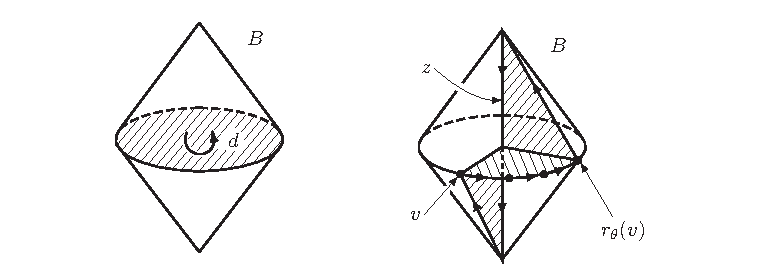
\includegraphics[width=.96\textwidth]{figures/8-9-2-3.pdf}
\caption*{图 8.9.2（左）与图 8.9.3（右）}
\end{figure}

\sourcepage{495}
$d,z$ 的承载集只交一点。严格地说，还需三角剖分，并将 $z$ 推到对偶一维骨架上，保持只有一个交点，这并不困难。由引理 8.9.3，$\{d\}\cdot\{z\}$ 为指定零维生成元的 $\pm1$ 倍。代入 $\{d\}=w$、$\{z\}=-k\beta_*w$，得到所需结论。\hfill$\square$

\entry{定理}{8.9.7}若 $L(n,k)$ 与 $L(n,\ell)$ 同伦等价，则必存在整数 $a$，使
\[k\equiv\pm a^2\ell\pmod n.\]

\textbf{证明：}设 $f:X\to Y$ 为同伦等价，取前一定理的生成元 $u,v$ 及顶维类 $\Lambda,\Lambda'$。写 $f^*v=au$。由 Bockstein 自然性及杯积自然性，
\begin{align*}
\pm[\ell]^{-1}f^*(\Lambda'_{(n)})
&=f^*(v\smile\beta^*v)
=f^*v\smile\beta^*(f^*v)\\
&=a^2(u\smile\beta^*u)=\pm a^2[k]^{-1}\Lambda_{(n)}.
\end{align*}
同伦等价使 $f^*\Lambda'=\pm\Lambda$，模 $n$ 后也如此，因此 $[\ell]^{-1}=\pm a^2[k]^{-1}$，即所需同余式。\hfill$\square$

\sourcepage{496}
此条件实际上既必要又充分；充分性由 J. H. C. Whitehead 证明。因此透镜空间是少数同胚分类与同伦分类都已解决的空间族（定理 4.14.15、注 4.14.16）。

Hurewicz 曾猜想：同伦等价的两个紧致流形应该同胚。二维时确实如此，但透镜空间给出三维反例。$L(7,1)$ 与 $L(7,2)$ 同伦等价，因为 $2\equiv3^2\pmod7$；但并不同胚，因为 $2\not\equiv\pm1$，且 $2\cdot1\not\equiv\pm1\pmod7$。

习题 3 表明，单凭 $H^*(L(n,k);\Z/n)$ 的环结构不足以作同伦分类，还需要 Bockstein。这是\emph{上同调运算}的一个例子。

\entry{定义}{8.9.8}类型为 $(p,q;G,G')$ 的上同调运算，是对每个拓扑偶定义的集合映射
\[\theta:H^p(X,A;G)\to H^q(X,A;G'),\]
并且相对于连续映射诱导的同态自然。\translatornote{原文目标系数有排印错误，这里按所声明的类型写作 $G'$。}

上同调运算赋予空间上同调远比环更丰富的结构。与透镜空间的例子一样，这些运算常能提供有价值的信息。

\sourcepage{496--497}
\subsection*{习题}
\begin{enumerate}
\item 若 $f:L(n,k)\to L(n,\ell)$ 的度为 $d$，证明存在整数 $a$，使 $kd\equiv\pm a^2\ell\pmod n$。
\item 利用本节结论、定理 4.14.15 及注 4.14.16，分别对 $L(7,k)$（$1\le k\le6$）和 $L(10,k)$（$k$ 与 $10$ 互素）作同胚分类及同伦分类。
\item 设 $X=L(n,k)$。
\begin{enumerate}[label=(\alph*)]
\item 若 $u_i$ 生成 $H^i(X;\Z/n)$，$i=1,2$，证明 $u_1\smile u_2$ 生成 $H^3(X;\Z/n)$。〔提示：先证明 $\beta^*:H^1\to H^2$ 是同构，从而存在一组这样的生成元。〕
\item 证明 $u_1\smile u_1$ 为零或阶为 $2$。\translatornote{原文此处写作 $u_1\smile u_2$，与 (a) 矛盾；按反交换律所适用的平方应为 $u_1\smile u_1$。}
\end{enumerate}
\item 对两个不同的自由链复形，各给出一个 Bockstein 同态的例子。
\end{enumerate}
